\documentclass[11pt,a4paper]{article}

\usepackage[utf8]{inputenc}
\usepackage[T1]{fontenc}
\usepackage[spanish]{babel}
\usepackage{amsmath}
\usepackage{graphicx}
\usepackage{placeins}
\usepackage{geometry}
\usepackage[expansion=false]{microtype}

\geometry{margin=2.5cm}

\title{Diagrama de estados: primera exploración}
\author{}
\date{}

\begin{document}
\maketitle

\section{Objetivo y protocolo}

Empezamos a explorar cómo cambian la morfología, el movimiento y la
organización colectiva de las células al variar la densidad $\rho$ y la
intensidad de la repulsión $\widetilde\kappa$. La idea de esta primera campaña
es ubicar regiones interesantes del diagrama, no identificar todavía una
transición crítica.

Simulamos $N=1000$ células inicialmente redondas, con posiciones aleatorias
y condiciones periódicas, para
\begin{equation}
\rho\in\{0.60,0.75,0.85,0.90,0.98\},\qquad
\widetilde\kappa\in\{0.75,1.50,2.50,4.00\}.
\end{equation}
En cada uno de los 20 puntos realizamos 64 simulaciones independientes hasta
$T=2000$, con $\Delta t=0.01$ y sin ruido aditivo. Mantuvimos los parámetros
fijados en las validaciones preliminares: $\lambda_{\rm core}=1$,
$AR_{\max}=2.7$, cinco intentos internos de elongación y
$\xi_{\rm safe}=0.8$. La morfología se actualiza en cada paso de integración.

Para resumir los estados usamos promedios temporales por realización en
$1500\leq t\leq2000$ y, después, promedios sobre las 64 realizaciones. Esta
ventana parece razonable para varios observables, pero no está garantizado
que describa un estado estrictamente estacionario en todos los puntos.

\section{Primeros resultados}

\subsection{Morfología y movimiento colectivo}

El atlas de la figura~\ref{fig:atlas} y los mapas de la
figura~\ref{fig:maps} muestran una separación bastante clara entre
regímenes. Para $\widetilde\kappa=0.75$ y $1.50$ encontramos una población
mayoritariamente elongada, con orden polar y polarización de velocidades
altos. También aparecen estructuras conectadas que ocupan una fracción
importante del sistema.

\begin{figure}[htbp]
    \centering
    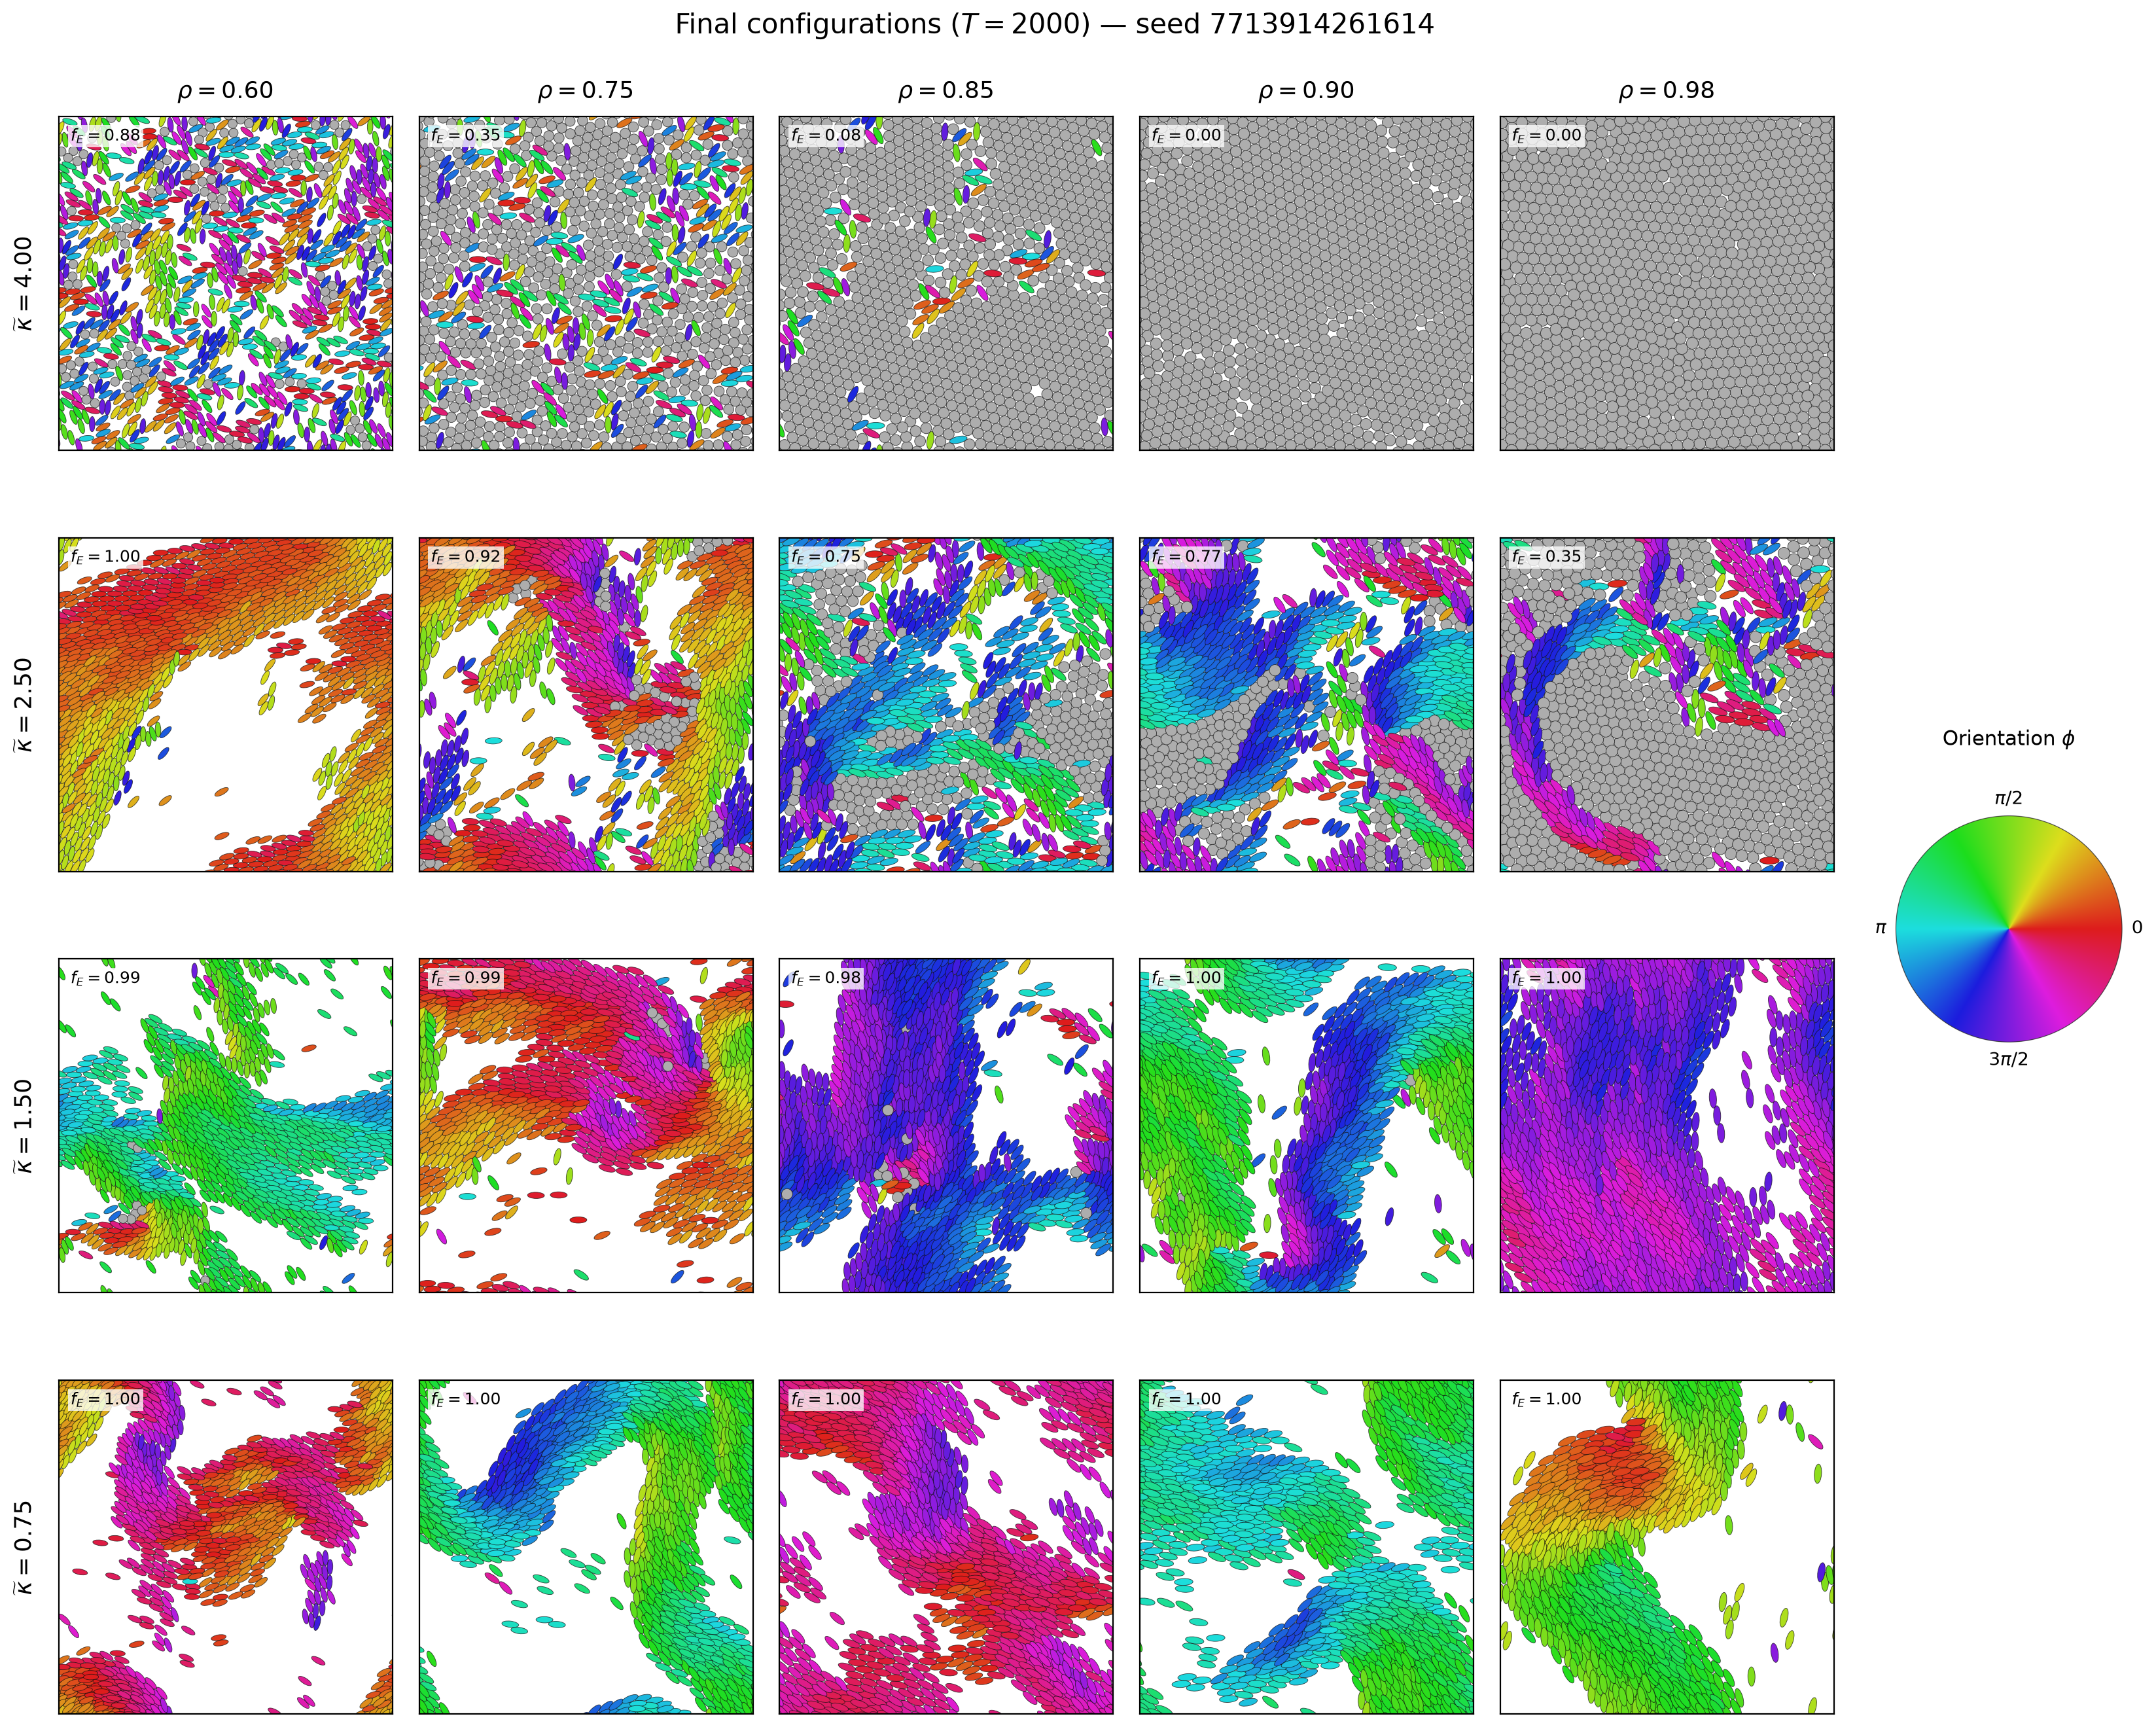
\includegraphics[width=0.96\textwidth]{../figures/final_configurations_atlas.png}
    \caption{Configuraciones finales ($T=2000$) de una realización compartida
    por los 20 puntos, con $\rho$ horizontal y $\widetilde\kappa$ creciente
    hacia arriba. Las células redondas están en gris y el color de las
    elongadas indica su orientación. El atlas es una referencia visual,
    no un promedio sobre realizaciones.}
    \label{fig:atlas}
\end{figure}

\begin{figure}[htbp]
    \centering
    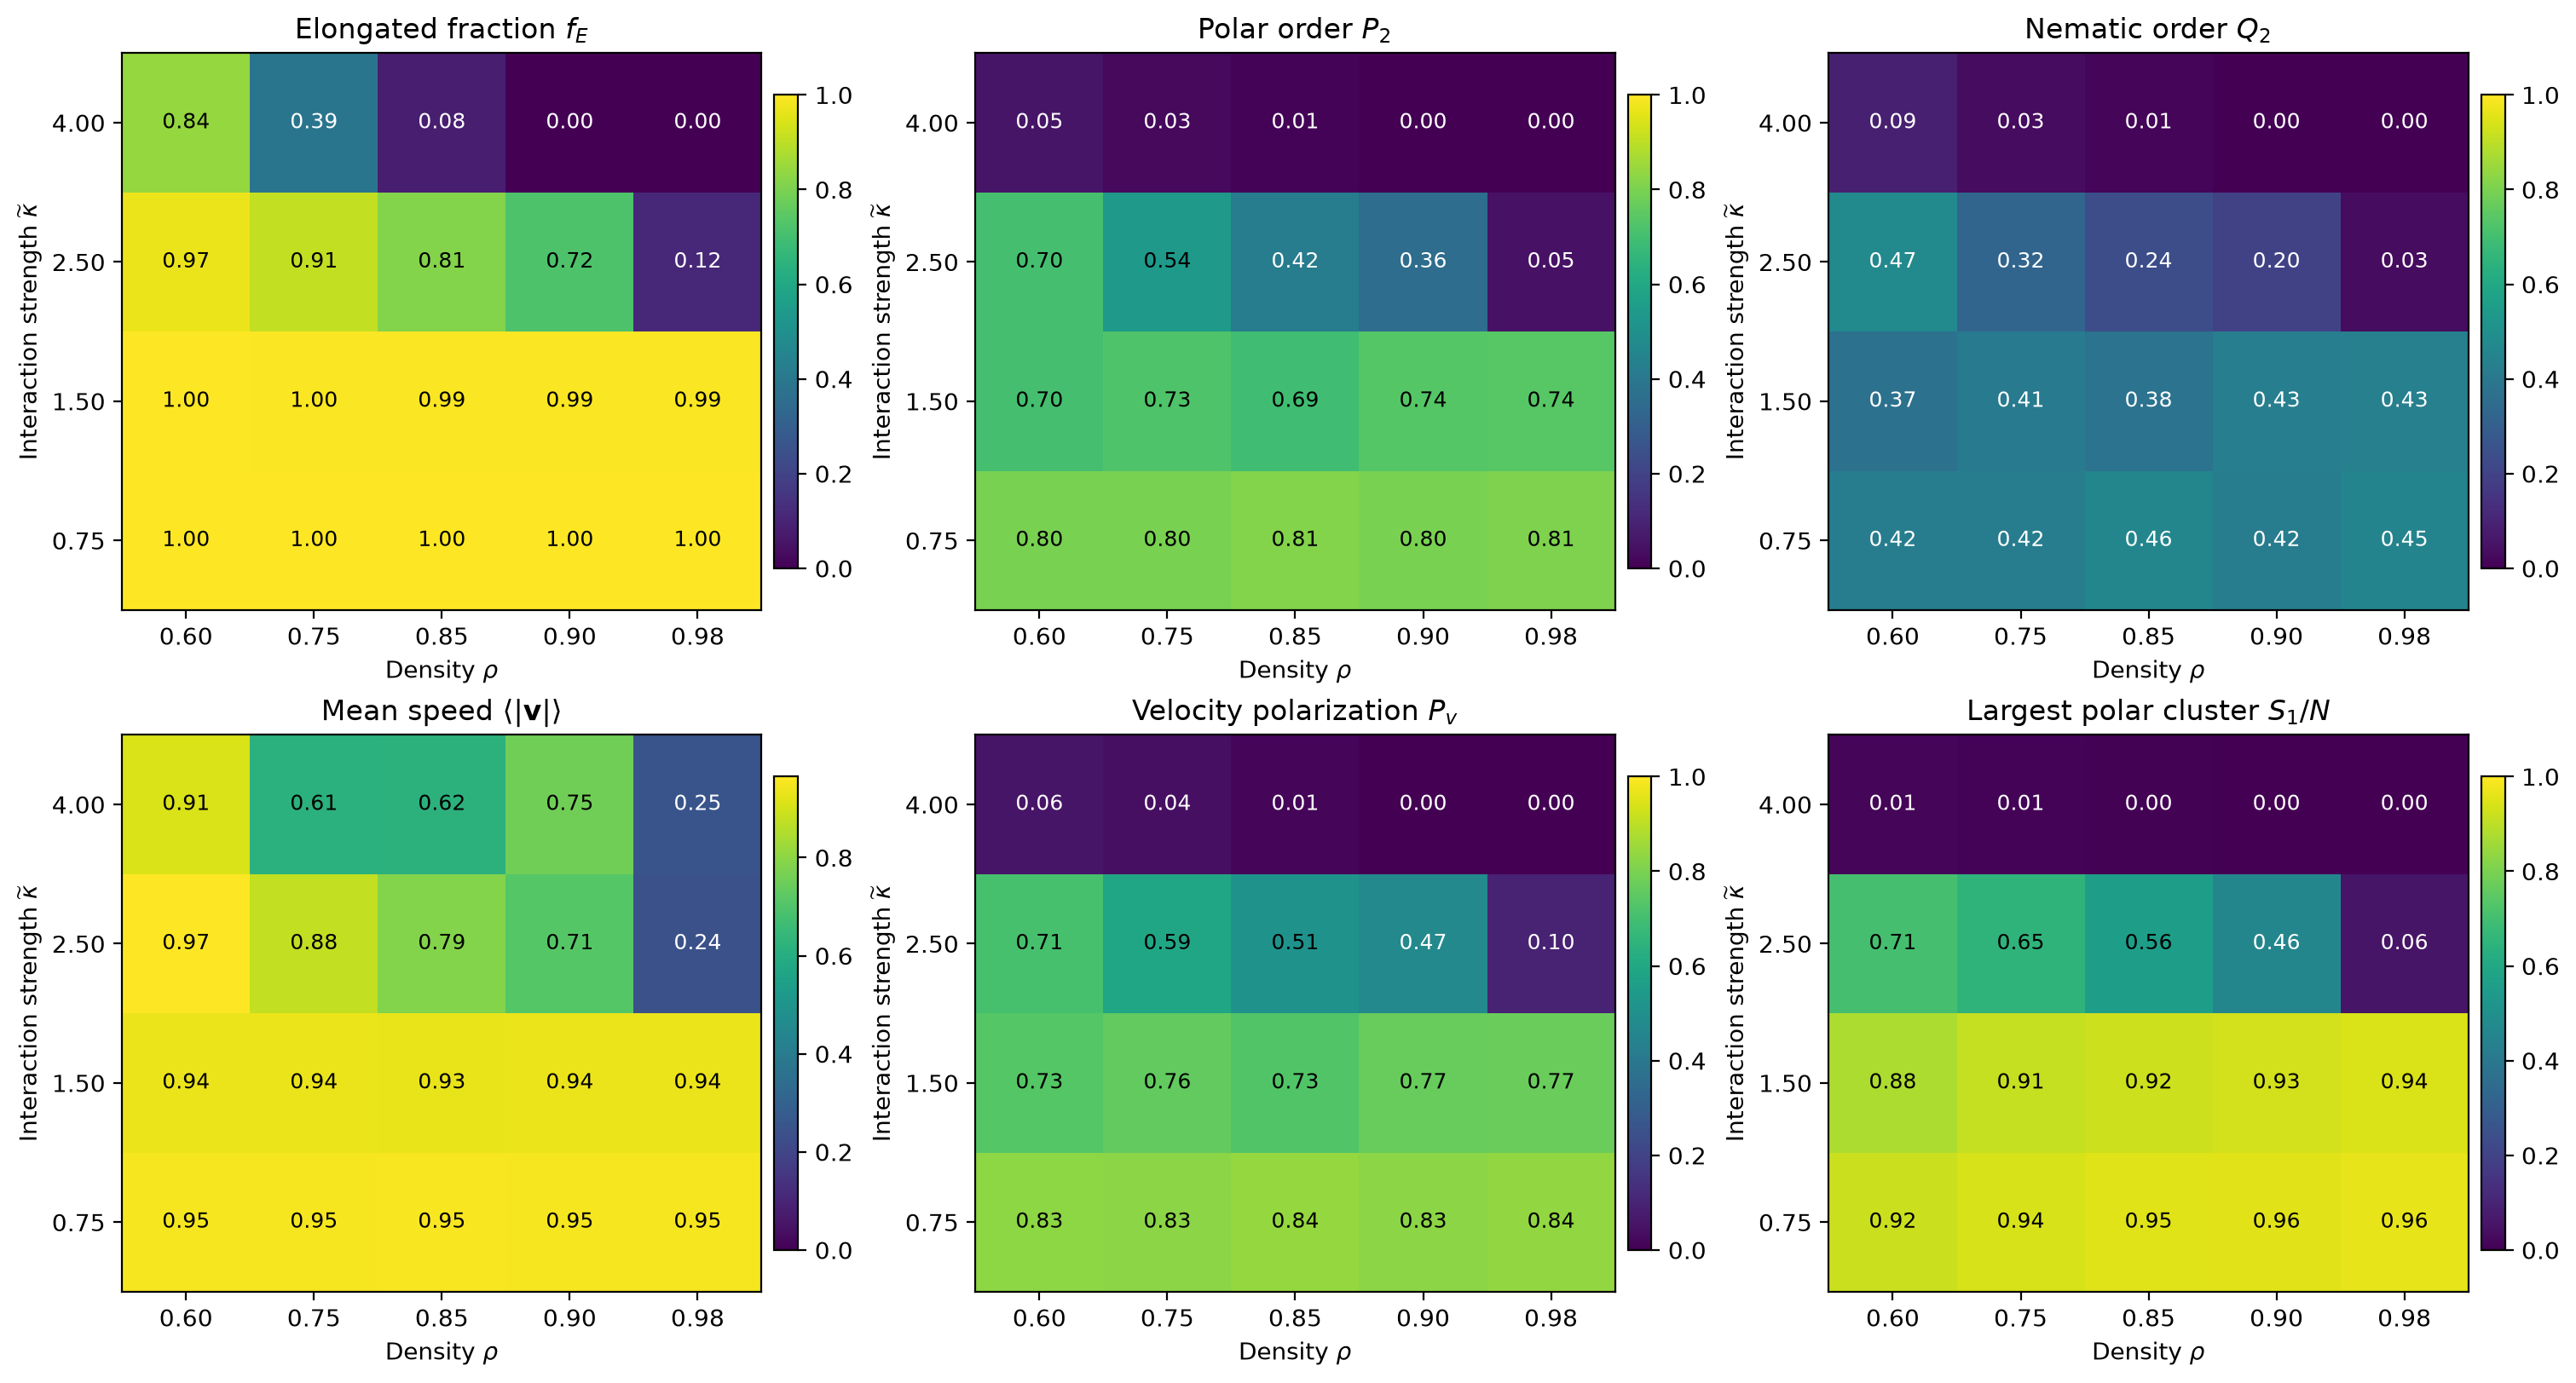
\includegraphics[width=0.96\textwidth]{../figures/state_diagram_main_maps.png}
    \caption{Promedios tardíos de la fracción elongada $f_E$, los órdenes
    polar y nemático normalizados por todas las células ($P_2$, $Q_2$),
    la velocidad mecánica media, la polarización de velocidades $P_v$ y
    la fracción $S_1/N$ del mayor cluster polar de células elongadas.
    Cada casillero corresponde a un punto simulado; no se interpola.}
    \label{fig:maps}
\end{figure}

La región de $\widetilde\kappa=2.5$ parece interesante. Al aumentar
$\rho$, aparecen más células redondas mientras disminuyen el orden polar
global, la coherencia de las velocidades y el tamaño relativo del mayor
cluster polar. No parece tratarse solamente de un cambio entre sistemas
completamente elongados y completamente redondos: hay puntos intermedios
en los que coexisten ambas morfologías y persisten estructuras colectivas.

También encontramos el caso complementario: para
$(\rho,\widetilde\kappa)=(0.60,4.00)$, gran parte de las células permanece
elongada, pero el orden polar y la conectividad polar global son bajos.

\subsection{Clusters y fluctuaciones}

Para estudiar conectividad usamos clusters de células elongadas conectadas
espacialmente y con orientaciones polares suficientemente próximas
(diferencia menor a $45^\circ$). Conviene mirar tanto $S_1/N$ como
$S_1/N_E$: el primero mide qué parte del sistema participa en el mayor
cluster y el segundo qué parte de la población elongada está conectada.
Esto evita atribuir automáticamente la caída de $S_1/N$ a una fragmentación:
también puede disminuir porque quedan menos células elongadas.

En $\widetilde\kappa=2.5$, las fluctuaciones entre realizaciones de $S_1/N$
son especialmente grandes alrededor de $\rho=0.90$, donde todavía hay una
fracción elongada apreciable. La figura~\ref{fig:fluct} muestra además que
las regiones de mayor variabilidad morfológica y de mayor variabilidad de
conectividad no coinciden exactamente.

\begin{figure}[htbp]
    \centering
    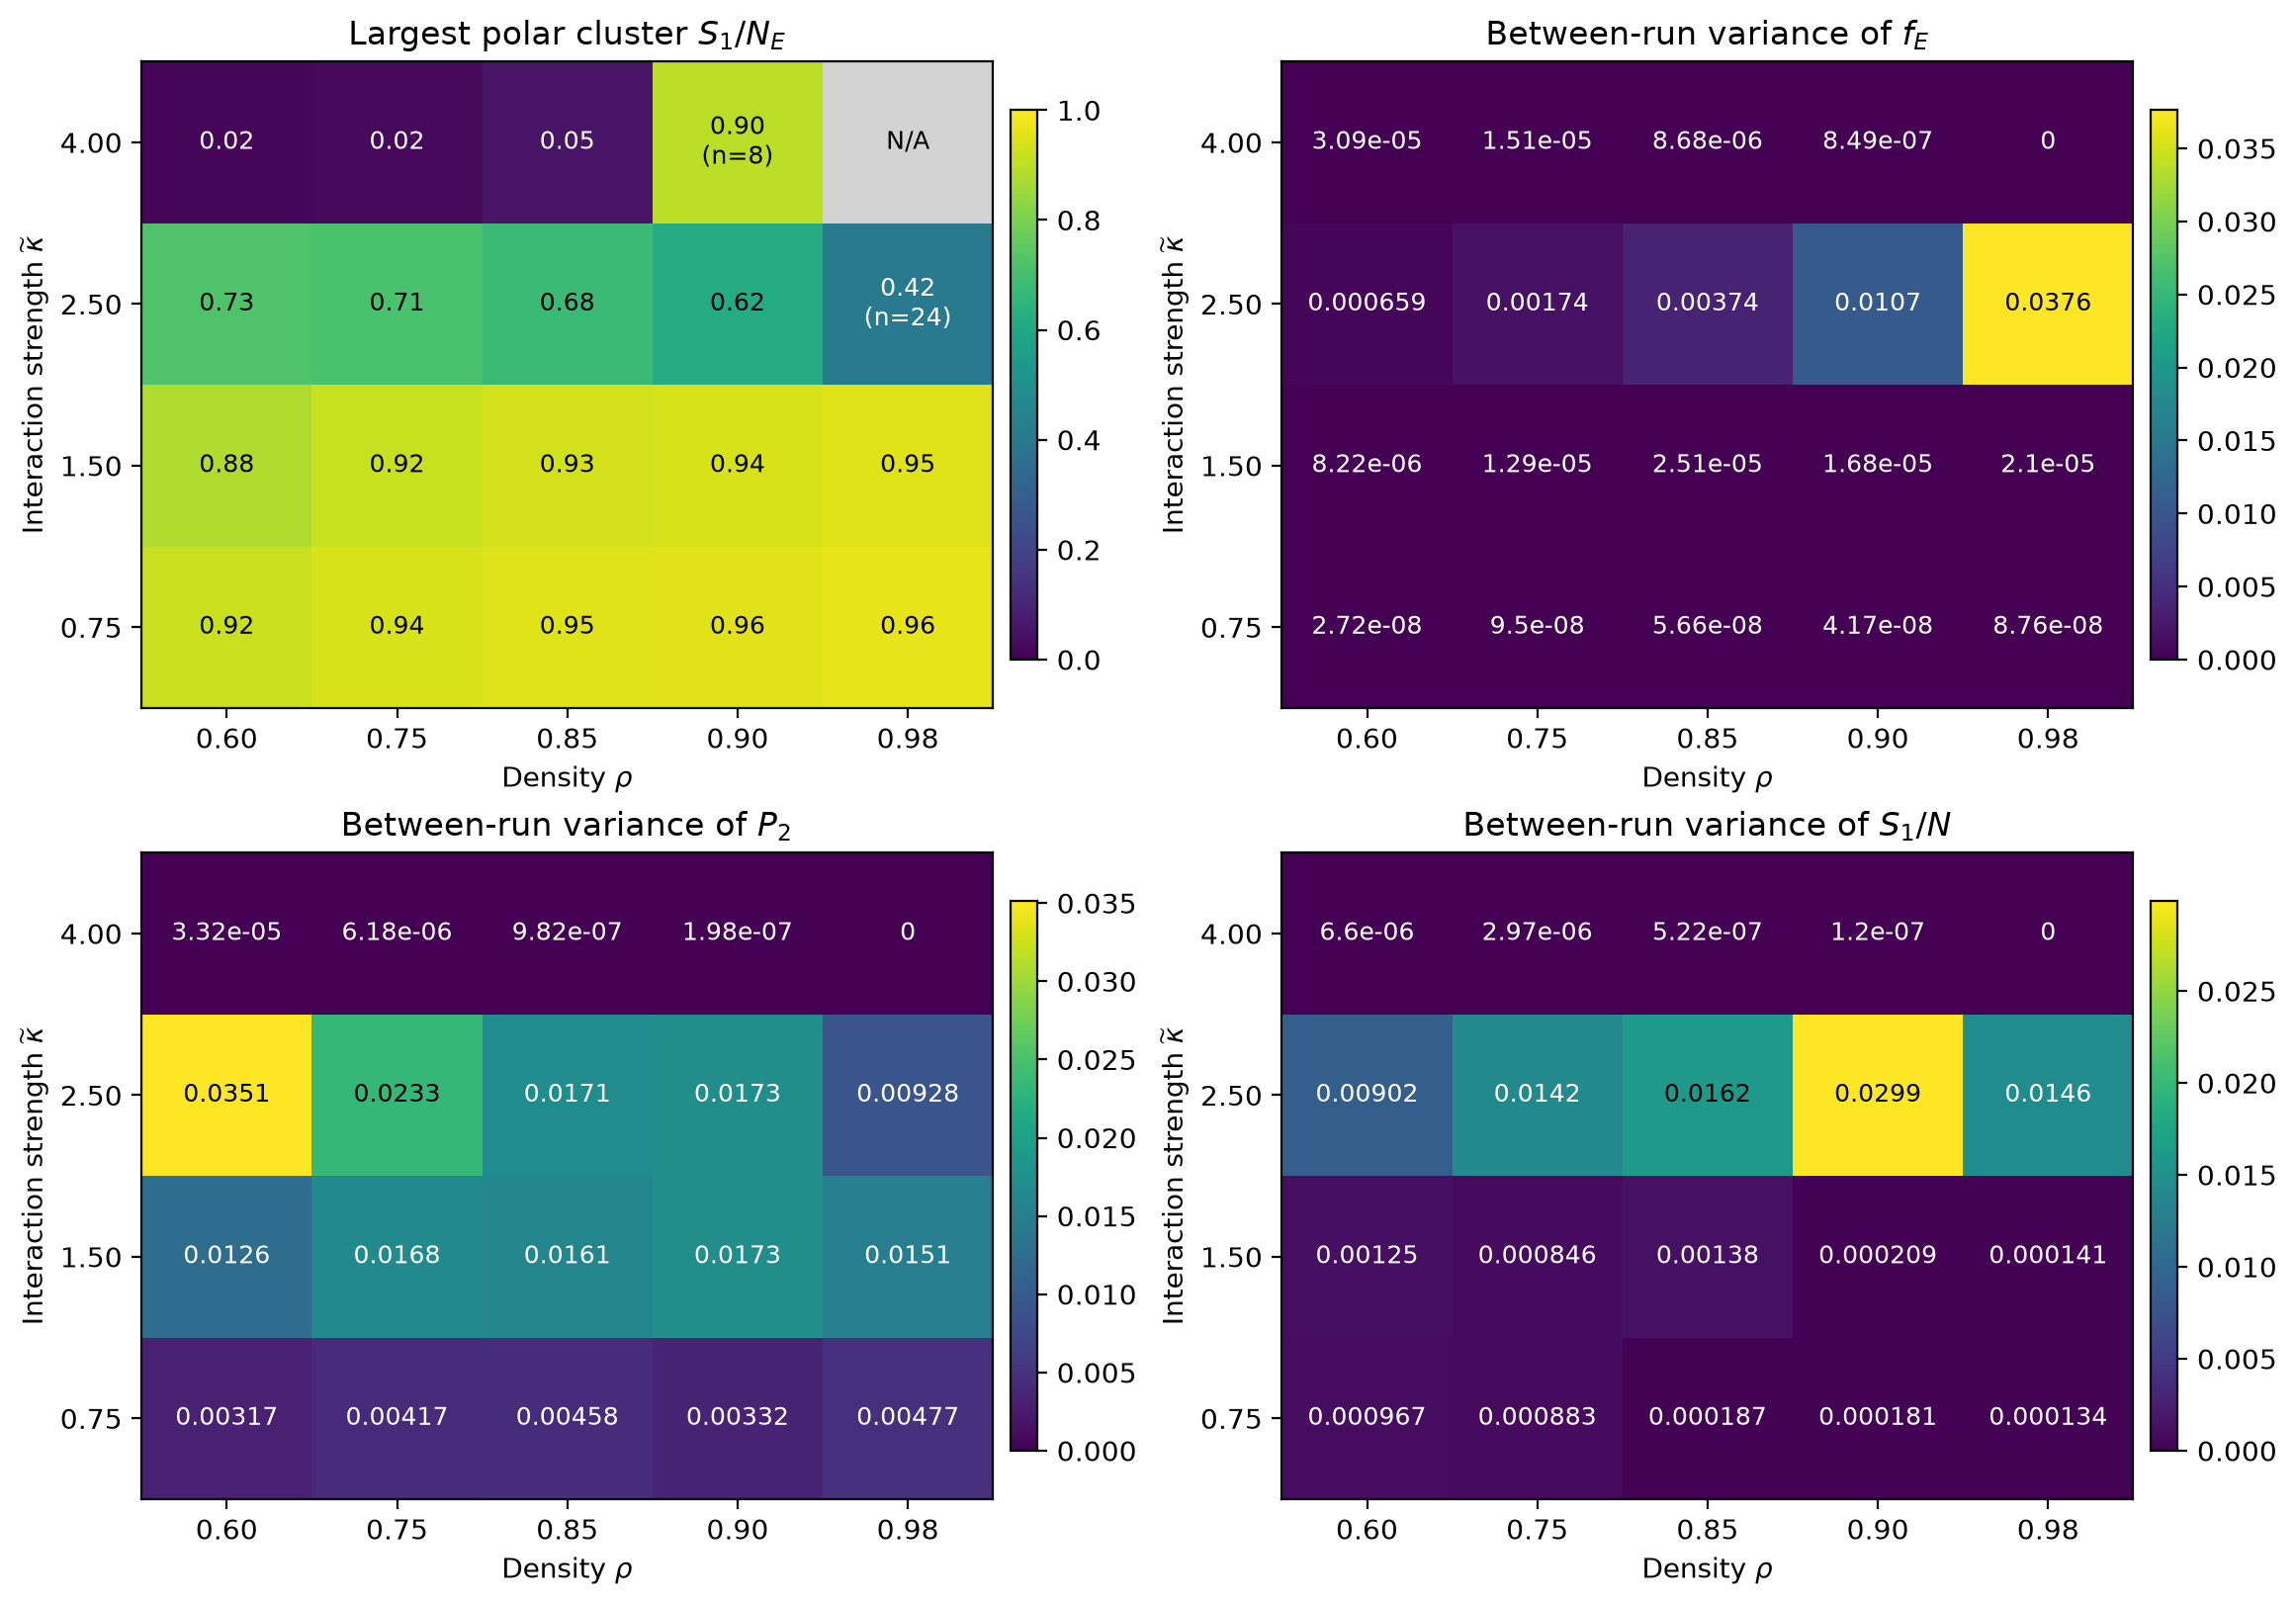
\includegraphics[width=0.95\textwidth]{../figures/state_diagram_fluctuations.png}
    \caption{Fracción del mayor cluster polar entre las células elongadas,
    $S_1/N_E$, y varianzas entre realizaciones de $f_E$, $P_2$ y $S_1/N$.
    Primero se promedia cada realización en la ventana tardía y luego se
    calcula la varianza entre realizaciones. $S_1/N_E$ se define solo cuando
    existen células elongadas.}
    \label{fig:fluct}
\end{figure}

Para ver un poco mejor de dónde viene esta variabilidad, la
figura~\ref{fig:distributions} muestra las distribuciones entre las 64
realizaciones para $\widetilde\kappa=2.5$. En $\rho=0.85$ y $0.90$
hay una dispersión apreciable del tamaño del mayor cluster, incluso
cuando muchas realizaciones mantienen una fracción elongada considerable.
En $\rho=0.98$, en cambio, se acumulan realizaciones con $f_E=0$ y
otras conservan valores positivos. Se observan
diferencias de conectividad para fracciones elongadas similares.

\begin{figure}[htbp]
    \centering
    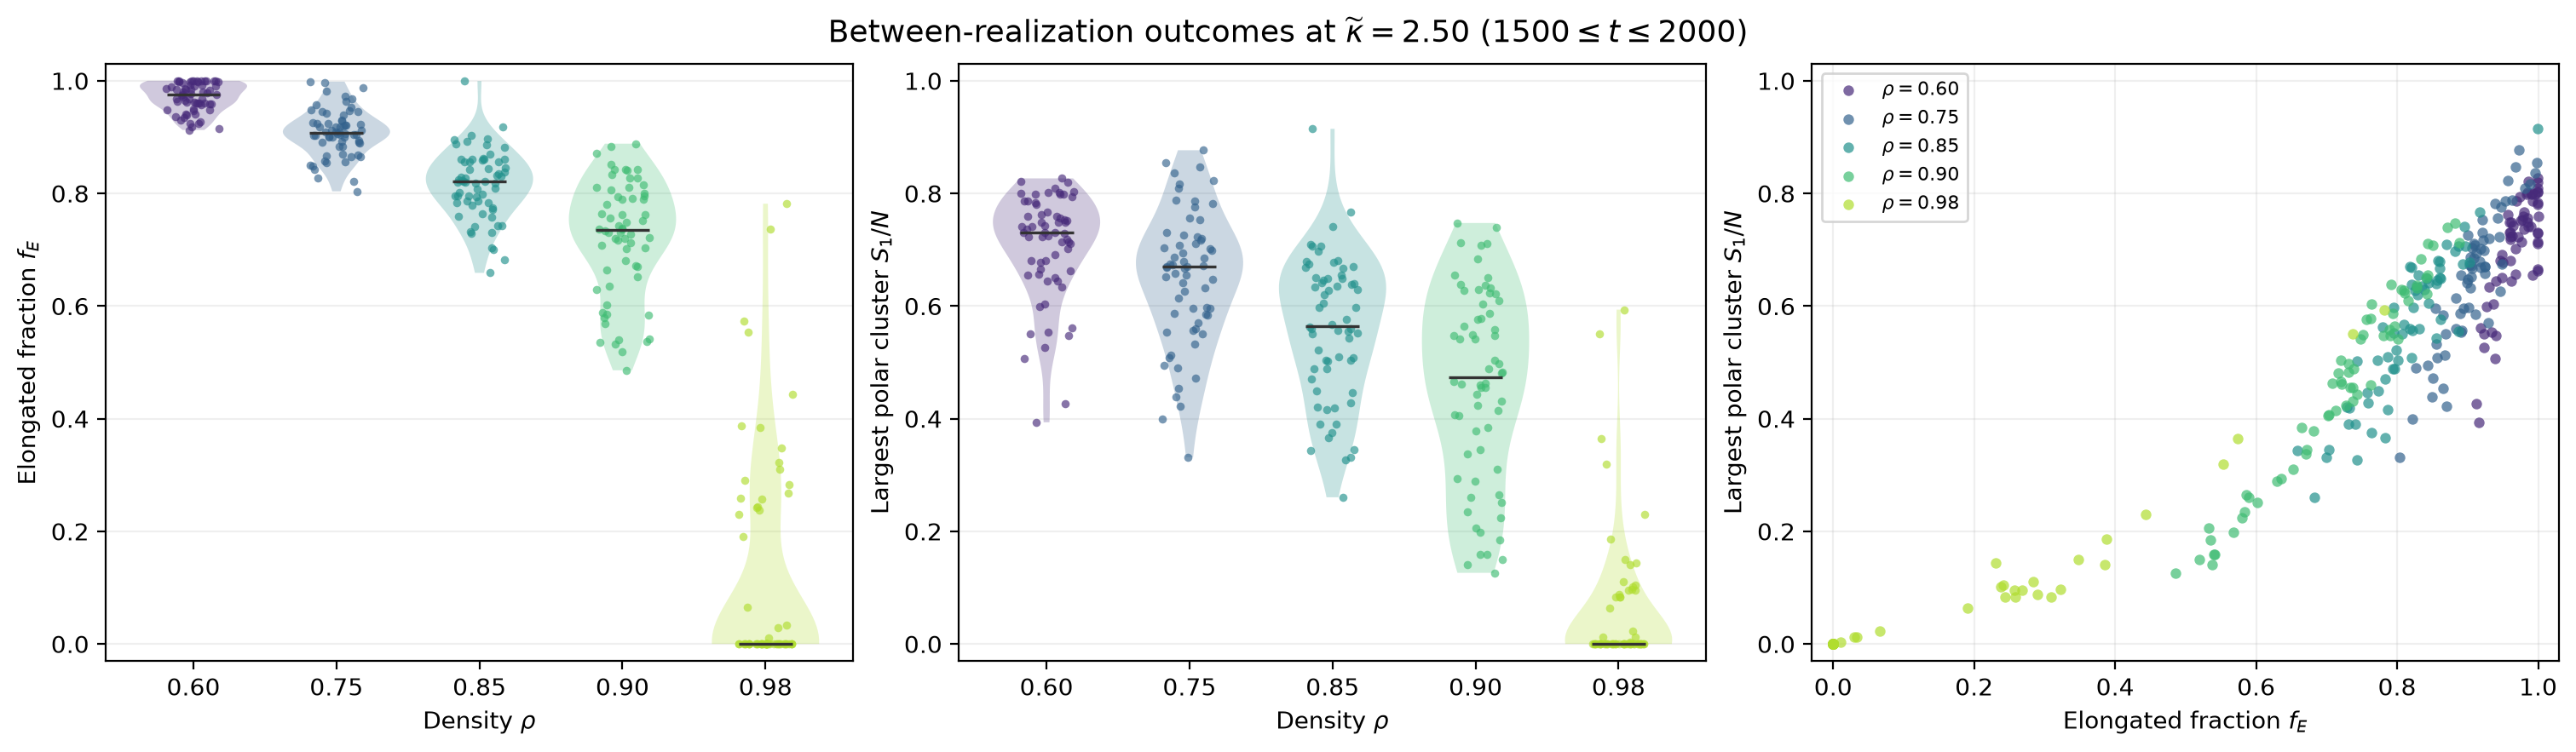
\includegraphics[width=0.96\textwidth]{../figures/state_diagram_distributions.png}
    \caption{Distribuciones entre realizaciones de la fracción elongada
    $f_E$ y del tamaño relativo del mayor cluster polar $S_1/N$ para
    $\widetilde\kappa=2.5$, junto con su relación realización por realización.
    Cada punto corresponde al promedio temporal de una realización en
    $1500\leq t\leq2000$; las formas suavizadas son una guía visual.}
    \label{fig:distributions}
\end{figure}

\FloatBarrier

\subsection{Una posible dinámica de atrapamiento}

Para $(\rho,\widetilde\kappa)=(0.98,2.5)$, 42 de las 64 realizaciones
terminan con $f_E(T)=0$, mientras que otras conservan células elongadas.
Las trayectorias individuales de la figura~\ref{fig:trajectories} muestran
que la media de ensamble esconde comportamientos diferentes entre
realizaciones. Algunas de las trayectorias que conservan elongación aún
presentan variaciones apreciables cerca de $T=2000$.

\begin{figure}[htbp]
    \centering
    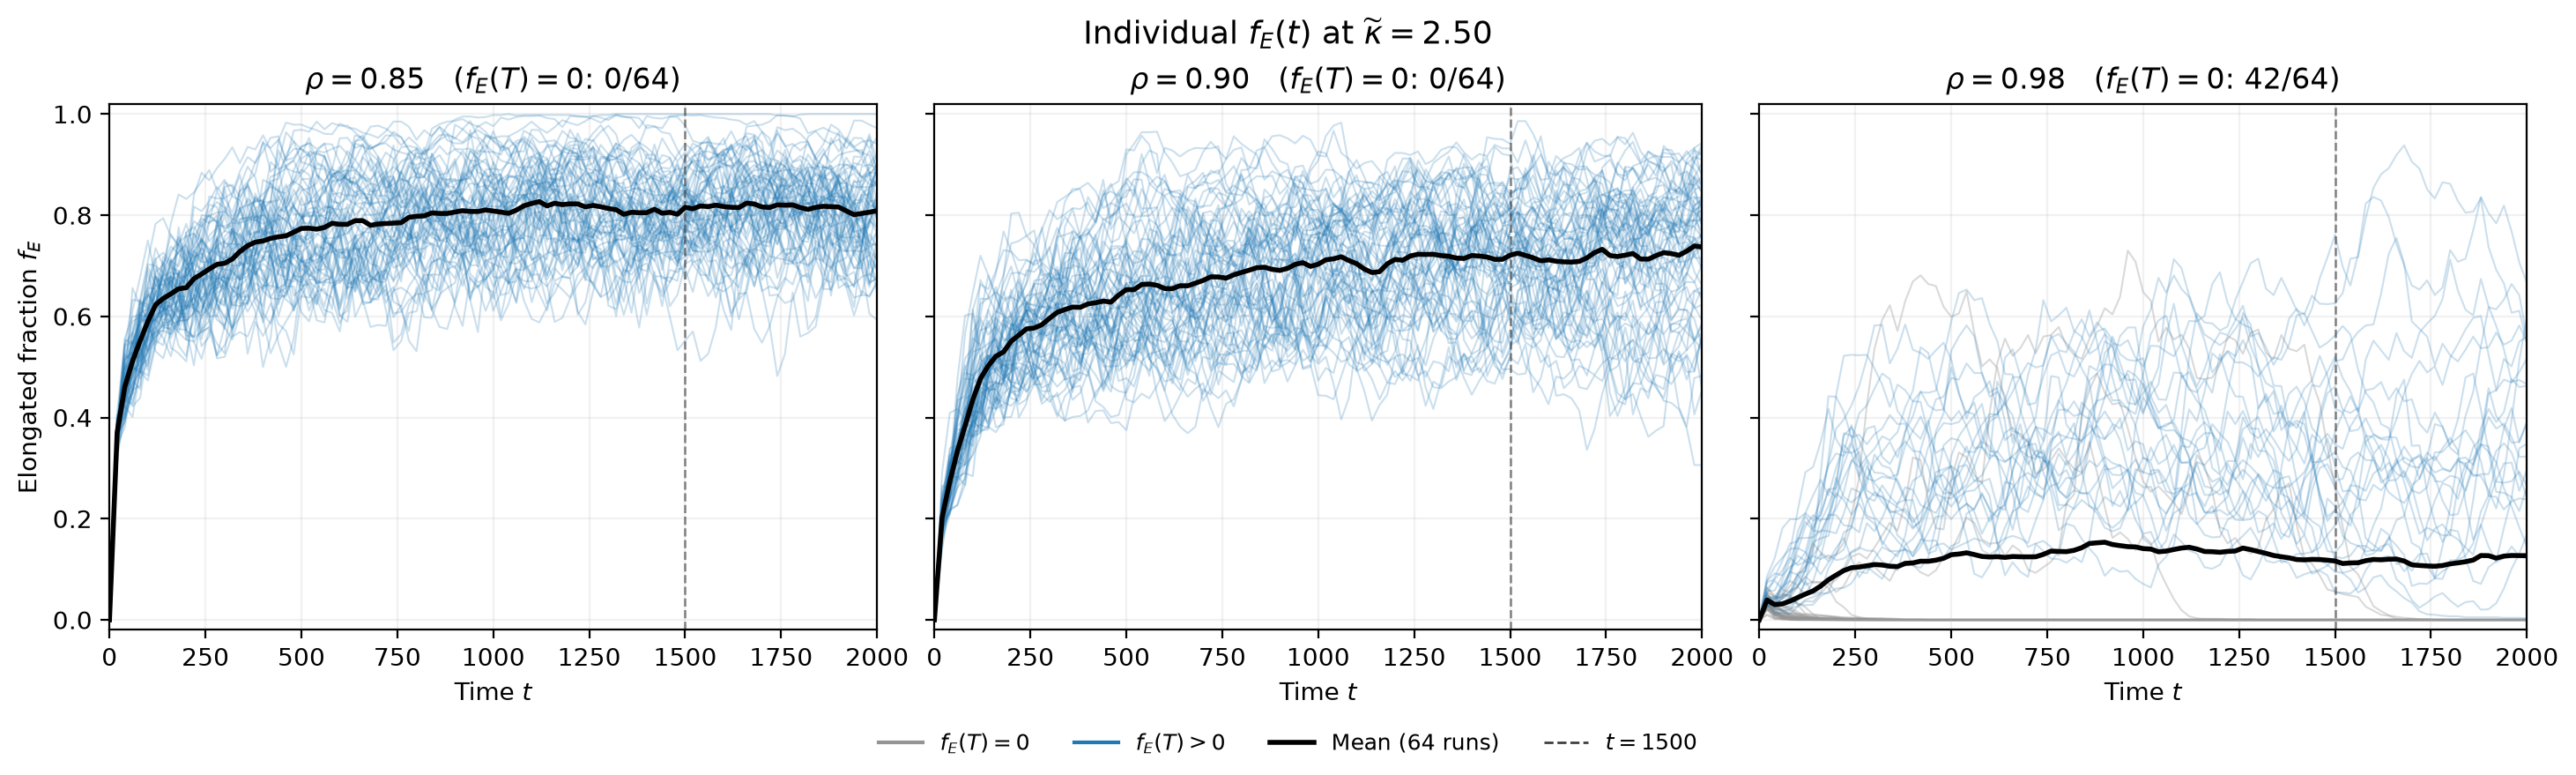
\includegraphics[width=0.96\textwidth]{../figures/state_diagram_individual_trajectories.png}
    \caption{Evolución de $f_E$ en las 64 realizaciones de tres densidades
    para $\widetilde\kappa=2.5$. Se distinguen las trayectorias que terminan
    completamente redondas de las que conservan células elongadas.}
    \label{fig:trajectories}
\end{figure}

El estado redondo parece ser absorbente (excepto en $t=0$ donde hay espacio). No lo es por construcción: las células redondas siguen
intentando elongarse.

\end{document}
